\documentclass[preview]{standalone}

\usepackage{color}
\usepackage{tikz}
\usetikzlibrary{positioning, graphs}
\usetikzlibrary{graphs.standard}
\usetikzlibrary{arrows.meta}


\begin{document}
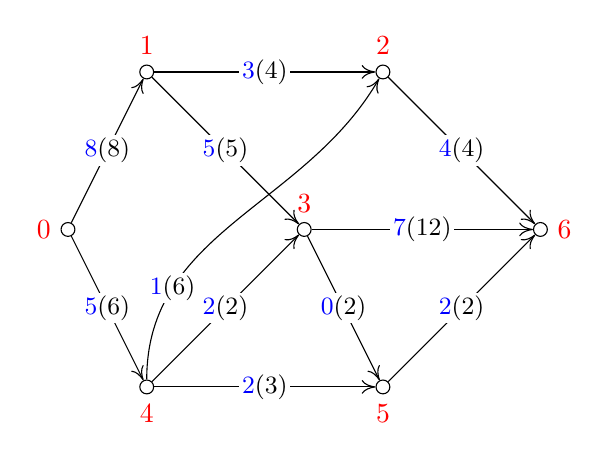
\begin{tikzpicture}
	[
		vertex/.style={draw,circle,inner sep = 0em, minimum size = 0.5em, fill=white},
		edgelabel/.style = {fill = white, inner sep = 0.1em, font=\small},
		nodelabel/.style = {color = red}
	]
	\node[vertex, label = {[nodelabel]left : 0}] (s) at (0, 0) {};
	\node[vertex, label = {[nodelabel]above : 1}] (a) at (1, 2) {};
	\node[vertex, label = {[nodelabel]above : 2}] (b) at (4, 2) {};
	\node[vertex, label = {[nodelabel]above : 3}] (c) at (3, 0) {};
	\node[vertex, label = {[nodelabel]below : 4}] (d) at (1, -2) {};
	\node[vertex, label = {[nodelabel]below : 5}] (e) at (4, -2) {};
	\node[vertex, label = {[nodelabel]right : 6}] (t) at (6, 0) {};
	
	\draw[-{>[length=5, width=5]}] (s) to node[edgelabel] {$\textcolor{blue}{8}(8)$} (a);
	\draw[-{>[length=5, width=5]}] (s) to node[edgelabel] {$\textcolor{blue}{5}(6)$} (d); 
	\draw[-{>[length=5, width=5]}, out = 90, in = -120] (d) to node[edgelabel, near start] {$\textcolor{blue}{1}(6)$} (b); 
	\draw[-{>[length=5, width=5]}] (a) to node[edgelabel] {$\textcolor{blue}{3}(4)$} (b);
	\draw[-{>[length=5, width=5]}] (a) to node[edgelabel] {$\textcolor{blue}{5}(5)$} (c);
	\draw[-{>[length=5, width=5]}] (b) to node[edgelabel] {$\textcolor{blue}{4}(4)$} (t);
	\draw[-{>[length=5, width=5]}] (c) to node[edgelabel] {$\textcolor{blue}{0}(2)$} (e);
	\draw[-{>[length=5, width=5]}] (c) to node[edgelabel] {$\textcolor{blue}{7}(12)$} (t);
	\draw[-{>[length=5, width=5]}] (d) to node[edgelabel] {$\textcolor{blue}{2}(2)$} (c);
	\draw[-{>[length=5, width=5]}] (d) to node[edgelabel] {$\textcolor{blue}{2}(3)$} (e);
	\draw[-{>[length=5, width=5]}] (e) to node[edgelabel] {$\textcolor{blue}{2}(2)$} (t);
\end{tikzpicture}
\end{document}